% !TeX program = lualatex
\documentclass[unicode, 11pt, aspectratio=169]{beamer}

% --- 日本語設定 ---
\usepackage{luatexja}
\usepackage[haranoaji]{luatexja-preset}

% --- デザイン・テーマ設定 ---
\usepackage{tikz}
\usetikzlibrary{shapes, positioning, calc}
\usetheme{Madrid}
\usecolortheme{default}
\usefonttheme{professionalfonts}

% --- 定理環境の設定 ---
\setbeamertemplate{theorems}[numbered]

% --- タイトル情報 ---
\title[DCJアルゴリズムの再実装]{Double-Cut-And-Join操作による\\ゲノム間距離に関する\\線形時間アルゴリズムの再実装}
\subtitle{2025年度 卒業論文}
\author{平田 智也}
\institute[慶應大・数理]{慶應義塾大学 理工学部 数理科学科\\小田研究室}
\date{2026年1月27日}

\begin{document}

% 1. タイトルスライド
\begin{frame}
    \titlepage
\end{frame}

% 3. 中身のスライド例
\section{はじめに}
\begin{frame}{研究背景と主な成果}
    \structure{研究の経緯}
    \begin{itemize}
        \item Oliveiraらのサーベイ論文\cite{oliveira2024}を調査
        \item 特に研究成果が豊富な \textbf{DCJ (Double Cut and Join)} に着目
        \item Bergeronら (2009)\cite{bergeron2009} の線形時間アルゴリズムを参照
    \end{itemize}

    \vspace{1em}
    \structure{本研究の動機}
    \begin{itemize}
        \item 既存のアルゴリズム\cite{bergeron2009}は記述が\textbf{過度に複雑}であり，
        \textbf{より簡素で分かりやすいアルゴリズム}を自分で実装することを目指した．
    \end{itemize}

    \vspace{1em}
    \structure{主な成果}
    \begin{itemize}
        \item DCJ距離および操作手順を$O(N)$で出力するアルゴリズムを，C言語で独自に実装した．
    \end{itemize}
\end{frame}

\section{理論的背景}

\begin{frame}{ゲノムの表現方法}
    \structure{ゲノムと染色体}
    \begin{itemize}
        \item ゲノムは\textbf{染色体}の集合であり，染色体は\textbf{遺伝子}の並び．
        \item 遺伝子は正負の整数で識別（$target$ ゲノムにおいて昇順）．
        \item 線形染色体 $\langle \dots \rangle$ と環状染色体 $( \dots )$．
    \end{itemize}

    \structure{端点 (extremity) と 隣接 (adjacency)}
    \begin{itemize}
        \item \textbf{端点}: 遺伝子 $g$ の右端 ($g$) と左端 ($-g$)．
        \item \textbf{隣接}: 接続された2つの端点の集合 $\{u, v\}$．
        \item 線形染色体の末端は\textbf{テロメア}\footnote{生物学において染色体の末端を保護する構造体に由来する名称} $o$との隣接 $\{o, x\}$ で表現．
    \end{itemize}
\end{frame}

\begin{frame}{具体例}
    $N=5$ の場合のゲノム表現:
    \begin{itemize}
        \item $A: \langle 1 \ -4 \rangle \ ( 3 \ -2 ) \ \langle 5 \rangle$
        \item $B: \langle 1 \ 2 \ 3 \rangle \ ( 4 \ 5 )$
    \end{itemize}

    \begin{center}
    \scalebox{0.8}{
    \begin{tikzpicture}[
        gene/.style={draw, rectangle, minimum height=1.0cm, minimum width=2.5cm, fill=orange!10, thick},
        lbl/.style={font=\small\bfseries}
    ]
        % Telomere 1
        \node (t1) at (0,0) {$\circ$};
        \node[below=0.1cm] at (t1) {\scriptsize テロメア};

        % Gene 1 [ -1 ... 1 ]
        \node[gene, right=0.3cm of t1] (g1) {};
        \node at (g1.west) [anchor=west, xshift=0.1cm] {$-1$};
        \node at (g1.center) {\Large\bfseries 1};
        \node at (g1.east) [anchor=east, xshift=-0.1cm] {$1$};

        % Connection 1
        \draw[thick] (t1) -- (g1);
        \node[blue, font=\Large, below=0.5cm] at ($(t1)!0.5!(g1.west)$) {$\{o, -1\}$};

        % Gene -4 [ 4 ... -4 ]
        \node[gene, right=0.3cm of g1] (g4) {};
        \node at (g4.west) [anchor=west, xshift=0.1cm] {$4$};
        \node at (g4.center) {\Large\bfseries -4};
        \node at (g4.east) [anchor=east, xshift=-0.1cm] {$-4$};

        % Connection 2
        \draw[thick] (g1) -- (g4);
        \node[blue, font=\Large, below=0.5cm] at ($(g1.east)!0.5!(g4.west)$) {$\{1, 4\}$};

        % Telomere 2
        \node[right=0.3cm of g4] (t2) {$\circ$};
        \node[below=0.1cm] at (t2) {\scriptsize テロメア};
        \draw[thick] (g4) -- (t2);
        \node[blue, font=\Large, below=0.5cm] at ($(g4.east)!0.5!(t2)$) {$\{-4, o\}$};


    \end{tikzpicture}
    }
    \end{center}

    隣接集合による表現:
    \begin{itemize}
        \item $A = \{ \{ o, -1 \}, \{ 1, 4 \}, \{ -4, o \}, \{ 3, 2 \}, \{ -2, -3 \}, \{ o, -5 \}, \{ 5, o \} \}$
        \item $B = \{ \{ o, -1 \}, \{ 1, -2 \}, \{ 2, -3 \}, \{ 3, o \}, \{ 4, -5 \}, \{ 5, -4 \} \}$
    \end{itemize}

    \vspace{0.5em}
    \small
    隣接集合による表現を用いることにより，
    線形であろうが円形であろうが統一的に染
    色体を扱うことができるようになる．
    また，DCJ操作も隣接に対する操作として扱うことができる．
\end{frame}

\begin{frame}{隣接グラフと例}

    \begin{definition}[隣接グラフ $AG(A,B)$]
        2つのゲノム $A, B$ のすべての隣接を頂点集合とし，
        共通する端点を持つ隣接同士の間にエッジを引いたグラフを隣接グラフ $AG(A,B)$ とする．
    \end{definition}
    \begin{center}
    \scalebox{0.7}{
    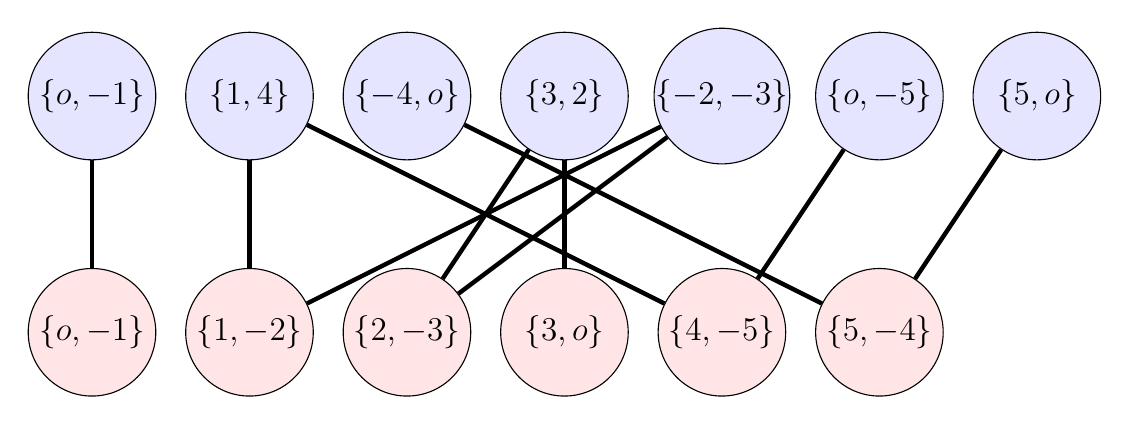
\begin{tikzpicture}[
        x = 2.0cm, y = 3.0cm, % 横幅を広げる
        every node/.style={circle, draw, minimum size=1.62cm, inner sep=0pt, font=\large},
        adjA/.style={fill=blue!10},
        adjB/.style={fill=red!10},
        edge/.style={-, ultra thick}
    ]
        % Genome A nodes (top row)
        \node[adjA] (a1) at (0, 0) {$\{ o, -1 \}$};
        \node[adjA] (a2) at (1, 0) {$\{ 1, 4 \}$};
        \node[adjA] (a3) at (2, 0) {$\{ -4, o \}$};
        \node[adjA] (a4) at (3, 0) {$\{ 3, 2 \}$};
        \node[adjA] (a5) at (4, 0) {$\{ -2, -3 \}$};
        \node[adjA] (a6) at (5, 0) {$\{ o, -5 \}$};
        \node[adjA] (a7) at (6, 0) {$\{ 5, o \}$};

        % Genome B nodes (bottom row)
        \node[adjB] (b1) at (0, -1) {$\{ o, -1 \}$};
        \node[adjB] (b2) at (1, -1) {$\{ 1, -2 \}$};
        \node[adjB] (b3) at (2, -1) {$\{ 2, -3 \}$};
        \node[adjB] (b4) at (3, -1) {$\{ 3, o \}$};
        \node[adjB] (b5) at (4, -1) {$\{ 4, -5 \}$};
        \node[adjB] (b6) at (5, -1) {$\{ 5, -4 \}$};

        % Edges
        \draw[edge] (a1) -- (b1); % -1
        \draw[edge] (a2) -- (b2); % 1
        \draw[edge] (a2) -- (b5); % 4
        \draw[edge] (a3) -- (b6); % -4
        \draw[edge] (a4) -- (b4); % 3
        \draw[edge] (a4) -- (b3); % 2
        \draw[edge] (a5) -- (b2); % -2
        \draw[edge] (a5) -- (b3); % -3
        \draw[edge] (a6) -- (b5); % -5
        \draw[edge] (a7) -- (b6); % 5
    \end{tikzpicture}
    }
    \end{center}

    隣接グラフ $AG(A,B)$ は，ゲノム $A$ の隣接集合とゲノム $B$ の隣接集合からなる二部グラフとなる．
    また，各頂点の次数は最大2であるため，隣接グラフは\textbf{パスまたはサイクルのみから構成される．}

\end{frame}

\begin{frame}{DCJ操作の定義と適用例}
    \begin{definition}[Double-Cut-And-Join]
        2つの隣接 $\{u, v\}$ と $\{x, y\}$ を切断し，
        新たに $\{u, x\}$ と $\{v, y\}$，
        または $\{u, y\}$ と $\{v, x\}$ として再結合する操作．
    \end{definition}
    隣接 $\{1, 4\}$ と $\{-2, -3\}$ に対してDCJ操作を適用し，$\{1, -2\}$ と $\{4, -3\}$ に組み替える．

    \begin{center}
    \scalebox{0.7}{
    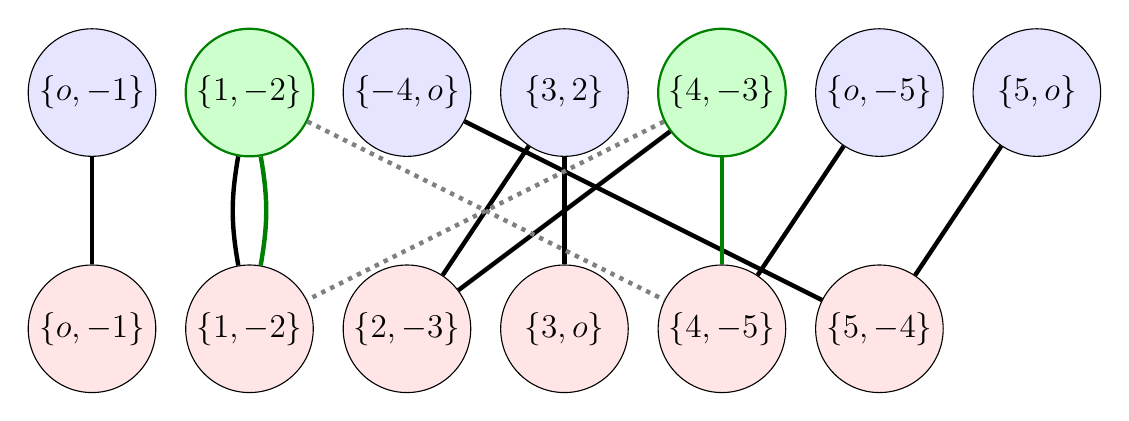
\begin{tikzpicture}[
        x = 2.0cm, y = 3.0cm,
        every node/.style={circle, draw, minimum size=1.62cm, inner sep=0pt, font=\large},
        adjA/.style={fill=blue!10},
        adjB/.style={fill=red!10},
        adjNew/.style={fill=green!20, draw=green!50!black, thick},
        edge/.style={-, ultra thick},
        edgeNew/.style={-, ultra thick, green!50!black}
    ]
        % Genome A nodes (top row)
        \node[adjA] (a1) at (0, 0) {$\{ o, -1 \}$};
        \node[adjNew] (a2) at (1, 0) {$\{ 1, -2 \}$};
        \node[adjA] (a3) at (2, 0) {$\{ -4, o \}$};
        \node[adjA] (a4) at (3, 0) {$\{ 3, 2 \}$};
        \node[adjNew] (a5) at (4, 0) {$\{ 4, -3 \}$};
        \node[adjA] (a6) at (5, 0) {$\{ o, -5 \}$};
        \node[adjA] (a7) at (6, 0) {$\{ 5, o \}$};

        % Genome B nodes (bottom row)
        \node[adjB] (b1) at (0, -1) {$\{ o, -1 \}$};
        \node[adjB] (b2) at (1, -1) {$\{ 1, -2 \}$};
        \node[adjB] (b3) at (2, -1) {$\{ 2, -3 \}$};
        \node[adjB] (b4) at (3, -1) {$\{ 3, o \}$};
        \node[adjB] (b5) at (4, -1) {$\{ 4, -5 \}$};
        \node[adjB] (b6) at (5, -1) {$\{ 5, -4 \}$};

        % Edges
        \draw[edge] (a1) -- (b1); % -1

        % Changed edges from a2 {1, -2}
        \draw[edge] (a2) to[bend right=10] (b2); % 1 in {1, -2}
        \draw[edgeNew] (a2) to[bend left=10] (b2);  % -2 in {1, -2}

        \draw[edge] (a3) -- (b6);

        \draw[edge] (a4) -- (b4); % 3
        \draw[edge] (a4) -- (b3); % 2

        % Changed edges from a5 {4, -3}
        \draw[edgeNew] (a5) -- (b5); % 4 in {4, -5}
        \draw[edge] (a5) -- (b3); % -3 in {2, -3}

        \draw[edge] (a6) -- (b5); % -5
        \draw[edge] (a7) -- (b6); % 5

        % --- Old connections (dotted) ---
        \draw[edge, dotted, gray] (a2) -- (b5);
        \draw[edge, dotted, gray] (a5) -- (b2);
    \end{tikzpicture}
    }
    \end{center}
\end{frame}

% --- DCJ距離の定義と問題提起 ---

\begin{frame}{DCJ距離の定義と本研究の課題}
    \begin{definition}[DCJ距離 $d_{\mathrm{DCJ}}$]
        2つのゲノム $A, B$ 間で，$A$ にDCJ操作を繰り返し適用すること
        により $B$ に変換するために必要な最小操作回数を
         $d_{\mathrm{DCJ}}(A,B)$ とする．
    \end{definition}

    \vspace{0.5em}
    本研究の主題は，任意の2つのゲノム $A, B$ に対して，この $d_{\mathrm{DCJ}}(A,B)$ を効率的に計算・出力するアルゴリズムを設計・実装することである．
\end{frame}

\begin{frame}{DCJ距離の下限}
    \begin{lemma}[DCJ距離の下限\cite{bergeron2006}]
        任意の2つのゲノム $A, B$ について，DCJ距離は以下を満たす：
        \[
            d_{\mathrm{DCJ}}(A,B) \ge N - \left( C + \frac{I}{2} \right)
        \]
    \end{lemma}
    \begin{alertblock}{成分の変化量に関する性質\cite{bergeron2006}}
        \begin{itemize}
            \item DCJ操作によってサイクル数 $C$ と奇数長パス数 $I$ が\textbf{同時に増減することはない}．
            \item サイクル数 $C$ が増減するときは，最大で $1$ しか変わらない ($\Delta C \in \{0, \pm 1\}$)．
            \item 奇数長パス数 $I$ が変化するときは，$2, 0, -2$ しか変わらない ($\Delta I \in \{0, \pm 2\}$)．
        \end{itemize}
    \end{alertblock}
\end{frame}

% --- アルゴリズムの正当性 ---

\begin{frame}{アルゴリズムの正当性の根拠}
    \begin{block}{整数性\cite{bergeron2006}}
        $C + I/2$ の変化量は常に $0$ または $\pm 1$ であり，DCJ操作ごとに距離 $d$ も整数として保たれる．
    \end{block}

    \begin{block}{最適性の保証\cite{bergeron2006}}
        任意の $A \neq B$ に対し，必ず $d$ を $1$ 減少させるDCJ操作が存在する．
        したがって，距離公式の下限値は実際に達成可能である．
    \end{block}

    したがって，Lemma 3と以上の議論より，次の定理が導かれる．
\end{frame}

\begin{frame}{DCJ距離公式とそれに基づく実装アプローチ1}

    {
    \setbeamercolor{block title}{bg=green!60!black,fg=white}
    \setbeamercolor{block body}{bg=green!10,fg=black}
    \begin{theorem}[DCJ距離公式\cite{bergeron2006}]
        2つのゲノム $A, B$ 間の最短のDCJ操作回数 $d_{\mathrm{DCJ}}(A,B)$ は，次式で与えられる：
        \[
            d_{\mathrm{DCJ}}(A,B) = N - \left( C + \frac{I}{2} \right)
        \]
        ここで $N$ は遺伝子数，$C$ はサイクル数，$I$ は奇数長パスの数である．
    \end{theorem}
    }
    \begin{block}{アプローチ1（距離公式に基づく実装）}
        初期状態の隣接グラフ $AG(A,B)$ を構築し，その成分（$C$ と $I$）を数え上げれば，操作シミュレーションを行わずとも距離 $d$ は求まる．
    \end{block}

    \begin{itemize}
        \item 具体的な操作手順は出力されないが，グラフ走査のみで完結する．
        \item \textbf{まずはこの手法を考案し，実装を行なった．}
    \end{itemize}
\end{frame}

\section{実装したアルゴリズム}

\begin{frame}{Bergeronらに基づく実装アプローチ2}
% \end{frame}

% \begin{frame}{実装アプローチ2：操作手順の導出}
    \begin{block}{アプローチ2（Bergeronら (2006)\cite{bergeron2006}に基づく貪欲法）}
        距離を $1$ 減少させる（$C + I/2$ を $1$ 増加させる）DCJ操作をGreedyに選択していき，グラフを動的に書き換えていく．
        その過程で操作手順も出力することができる．
    \end{block}

    \begin{itemize}
        \item 隣接の繋ぎ変えを追跡することで，具体的な変形操作の系列を出力可能．
        \item \textbf{距離計算の実装に続き，こちらも実装を行なった．}
    \end{itemize}

    \vspace{0.5em}
    \begin{alertblock}{計算量について}
        いずれの手法についても，入力サイズ $N$ に対して線形時間 $O(N)$ で動作するアルゴリズムとして実装できた．
    \end{alertblock}
\end{frame}

% 4. 実装に関するページ
\section{実装と今後の課題}
\begin{frame}{DCJ距離アルゴリズム実装と課題}
    上述のアプローチ1，2をC言語により実装した．
    実行時間のオーダーはどちらも線形時間 $O(N)$ である．
    ゲノム間の隣接グラフなどを走査し，
    アプローチ1は距離のみ，アプローチ2は距離と操作手順を出力する．

    詳細なソースコードは以下のGitHubリポジトリで公開している：
    \begin{itemize}
        \item \url{https://github.com/hiratannnnnn/dcj_bergeron.git}
    \end{itemize}

    \vspace{1em}
    \structure{課題}
    \begin{itemize}
        \item 現状の実装ではテキスト入力のパースを用いているため，
        遺伝子番号の桁数に起因して，
        入力時に見かけ上の対数的なコストが発生している．
        固定長整数の形式にするなど，
        桁数に依存しないようにすれば，
        厳密な線形時間化が可能になる．
    \end{itemize}
\end{frame}

\begin{frame}[allowframebreaks]{参考文献}
\begin{thebibliography}{9}

	\bibitem{bergeron2006}
	A. Bergeron, J. Mixtacki, and J. Stoye, ``A unifying view of genome rearrangements,'' in: \textit{Proceedings of WABI 2006}, LNBI, vol. 4175, Springer Verlag, 2006, pp. 163--173.

	\bibitem{bergeron2009}
	A. Bergeron, J. Mixtacki, and J. Stoye, ``A new linear time algorithm to compute the genomic distance via the double cut and join distance,'' \textit{Theoretical Computer Science}, 410 (2009), pp. 5300--5316.

	\bibitem{hp1995}
	S. Hannenhalli and P. A. Pevzner, ``Transforming men into mice (polynomial algorithm for genomic distance problem),'' in: \textit{Proceedings of FOCS 1995}, IEEE Press, 1995, pp. 581--592.

	\bibitem{oliveira2024}
	A. R. Oliveira, K. L. Brito, A. O. Alexandrino, G. Siqueira, U. Dias, and Z. Dias, ``Rearrangement Distance Problems: An Updated Survey,'' \textit{CSUR}, 2024.

\end{thebibliography}
\end{frame}

\end{document}
